%
% Chapter 5
%
\chapter{CSE Analog Components}
\section{Analog Circuit}
In order to develop a better testing procedure for the current amplifier circuits as well as begin development of the next generation, some exploration of the initial designers' writing was required. Analog output from the CSE was addressed to each pixel of the IRSP. Due to the sensitive nature of digital-to-analog communications and the unique load requirements of the system the entire system architecture had to be measured and mapped out. To do so, the system was split into various sections representing gain and load stages. \cite{marks}. The first stage (DAC Buffer) was responsible for terminating the differential output of the DAC and turning it into a single-ended signal. The next stage was the Cable Driver, a gain stage which was responsible for driving interface board communication and ribbon cable signals. This stage provides some, but not all of the voltage gain required to drive the RIIC from 0-5V. The ribbon cables would output to the final stage known as the Dewar Driver. This stage provides the remainder of the gain required to drive the RIIC at 5V. The Dewar output stage was a 10nF load and required a 0-10V swing from the amplifiers. \par
\begin{figure}[!htb]
	\includegraphics*[]{analog_stages}
	\centering
	\caption{High-level schematic of the analog gain \& impedance stages}
	\centering
\end{figure}
\section{Understanding the Requirements}
To properly test, validate and repair the amp cards, one requires an understanding of the card's place in the system. The card was responsible for passing digital-to-analog converted signals with 16-bit resolution at high speeds, and any issues would be directly visible in the projected video. The amp card received inputs from a 16-bit DAC with a 250 Megasamples per second output \cite{marks}. For digital information to be properly decoded as an analog signal, the converter must settle on values at an acceptable speed with negligible margin of error. As bit resolution increases, the margin of error should decrease.\par

\section{Settling Time}
In any digital-to-analog system, designers must account for physical characteristics of electronics. Every DAC has a delay between input and response, known as Delay Time. The DAC then enters a Slewing period, where it tries to approach the target current or voltage output as fast as possible (current level in the case of our specific DAC). As the DAC approaches the target, slope decreases and the DAC oscillates between over- and under-estimates of the value until finally settling on a DC output. While an ideal DAC will settle on a precise output, most DACs will continue to oscillate between values if it is unable to discern their mean, especially in practical situations. The mathematical account of this phenomenon is called the Error Band. \par
\begin{figure}[!htb]
	\includegraphics*[width=15cm]{error_band}
	\centering
	\caption{Example DAC output}
	\centering
\end{figure}
\section{Error Band}
The maximum acceptable error band is notated as
\begin{math}
	\frac{Vout}{2^n}
\end{math}
where Vout represents the maximum voltage output of the device and N represents the desired bit resolution. An 8-bit system with 4V max output, for example, has an error band of 
\begin {math}
	\frac{4V}{2^8}=0.0156V
\end{math}
The settling time is the time it takes for our analog system to be bounded by this error band. A smaller error band makes calculating the final value more difficult for the device.

\section{PCB}
The amp card was designed to encompass the first and second stages (DAC Buffer/Cable Driver). Prototype and final PCB layouts are attached below. The load and bandwidth requirements meant that the amplifiers had to have a high slew rate (reflected as rise time in the Dewar) and bandwidth. These design choices were the basis for the v2 redesign which will be discussed later. Each amp card contained two amplifiers, and each amplifier had their own ground planes which were unified at the DAC input and interface board output connectors. This is a common design choice meant to eliminate cross-talk between ground planes of sensitive analog components at high speeds. Each amplifier component was a quad amplifier, but only the first two were used in the design. While this decision was also made out of concern for cross-talk, the unusued pins wasted quite a bit of space and were one of the first motivations for a new PCB in Nessie2. The amplifier card was initially designed as a 2-layer PCB which proved to be insufficient for power delivery and signal integrity \cite{marks}. The board was redesigned to a 4-layer version and extensively tested to ensure the previous concerns were fixed. \par
\begin{figure}[!htb]
	\includegraphics*[width=15cm]{amp_prototype}
	\centering
	\caption{Prototype Amp Layout}
	\centering
\end{figure}
\begin{figure}[!htb]
	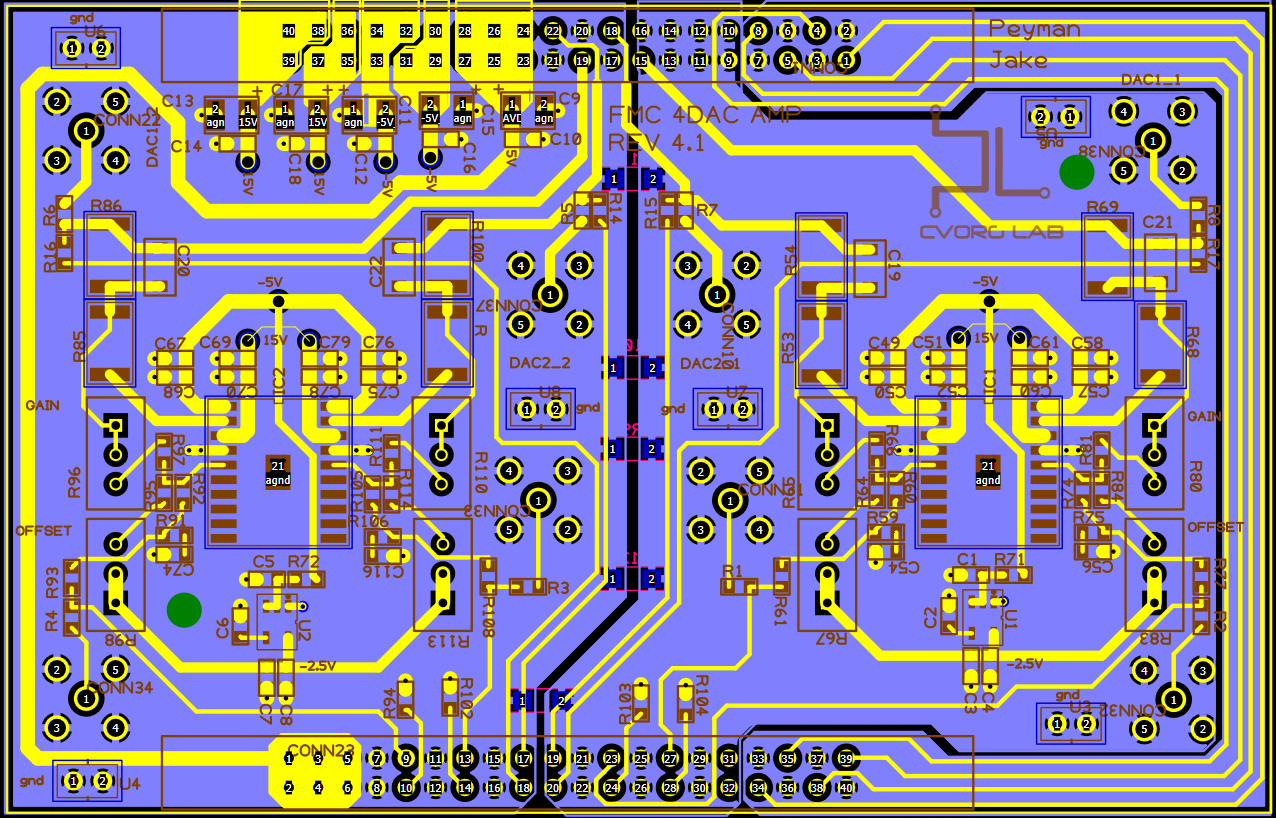
\includegraphics[width=15cm]{amp_final}
	\centering
	\caption{Final Amp Layout}
	\centering
\end{figure}



